\chapter{NoSQL: vergelijkende studie}
\label{nosql_survey}

\section{Methodologie}

Omwille van het enorme aanbod aan NoSQL en NewSQL systemen was een exhaustieve studie niet haalbaar. Deze vergelijkende studie behandelt de populairste datastores in een aantal relevante categorie\"en, namelijk document stores, columnar stores en NewSQL stores. Key-value stores en graph databases komen niet aan bod, aangezien hun datamodellen niet geschikt zijn voor de toepassing in kwestie. De uiteindelijke selectie werd gemaakt volgens criteria vergelijkbaar met die in \cite{grolinger2013data}, met de ranking van DB-Engine Ranking \cite{db_engine_rank} als maat voor de populariteit.\\

Deze ranglijst tracht populariteit te meten op basis van enkele parameters, zoals aantal vermeldingen op websites, algemene interesses volgens Google Trends, frequentie van technische discussies op fora zoals StackOverflow, vacatures i.v.m. de technologie en vermeldingen in professionele profielen op sites zoals LinkedIn. De resulterende selectie bestaat uit de document stores MongoDB en CouchBase Server, wide columnar stores Cassandra en HBase en NewSQL database VoltDB. Er bestaat al een uitbreiding van de DNA sequencing pijplijn die het ExaScience Life Lab gebruikt om MongoDB  databanken als in- en/of uitvoer te gebruiken voor de pijplijn. Dit maakt MongoDB uiteraard nog relevanter. Ten laatste werd ook NewSQL query engine Cloudera Impala in de studie betrokken wegens expliciete interesse van onderzoekers in het eerder vernoemde lab. Deze 6 systemen vergeleek ik 
%TODO ik?
vervolgens op een aantal voor high performance computing relevante eigenschappen zoals indexeringsmechanismen, interfaces naar de gebruiker en API's, distributiestrategie, concurrency controle en consistentiemodel. Tabel \ref{survey_tabel} geeft een overzicht weer van de bestudeerde systemen.

\begin{landscape}
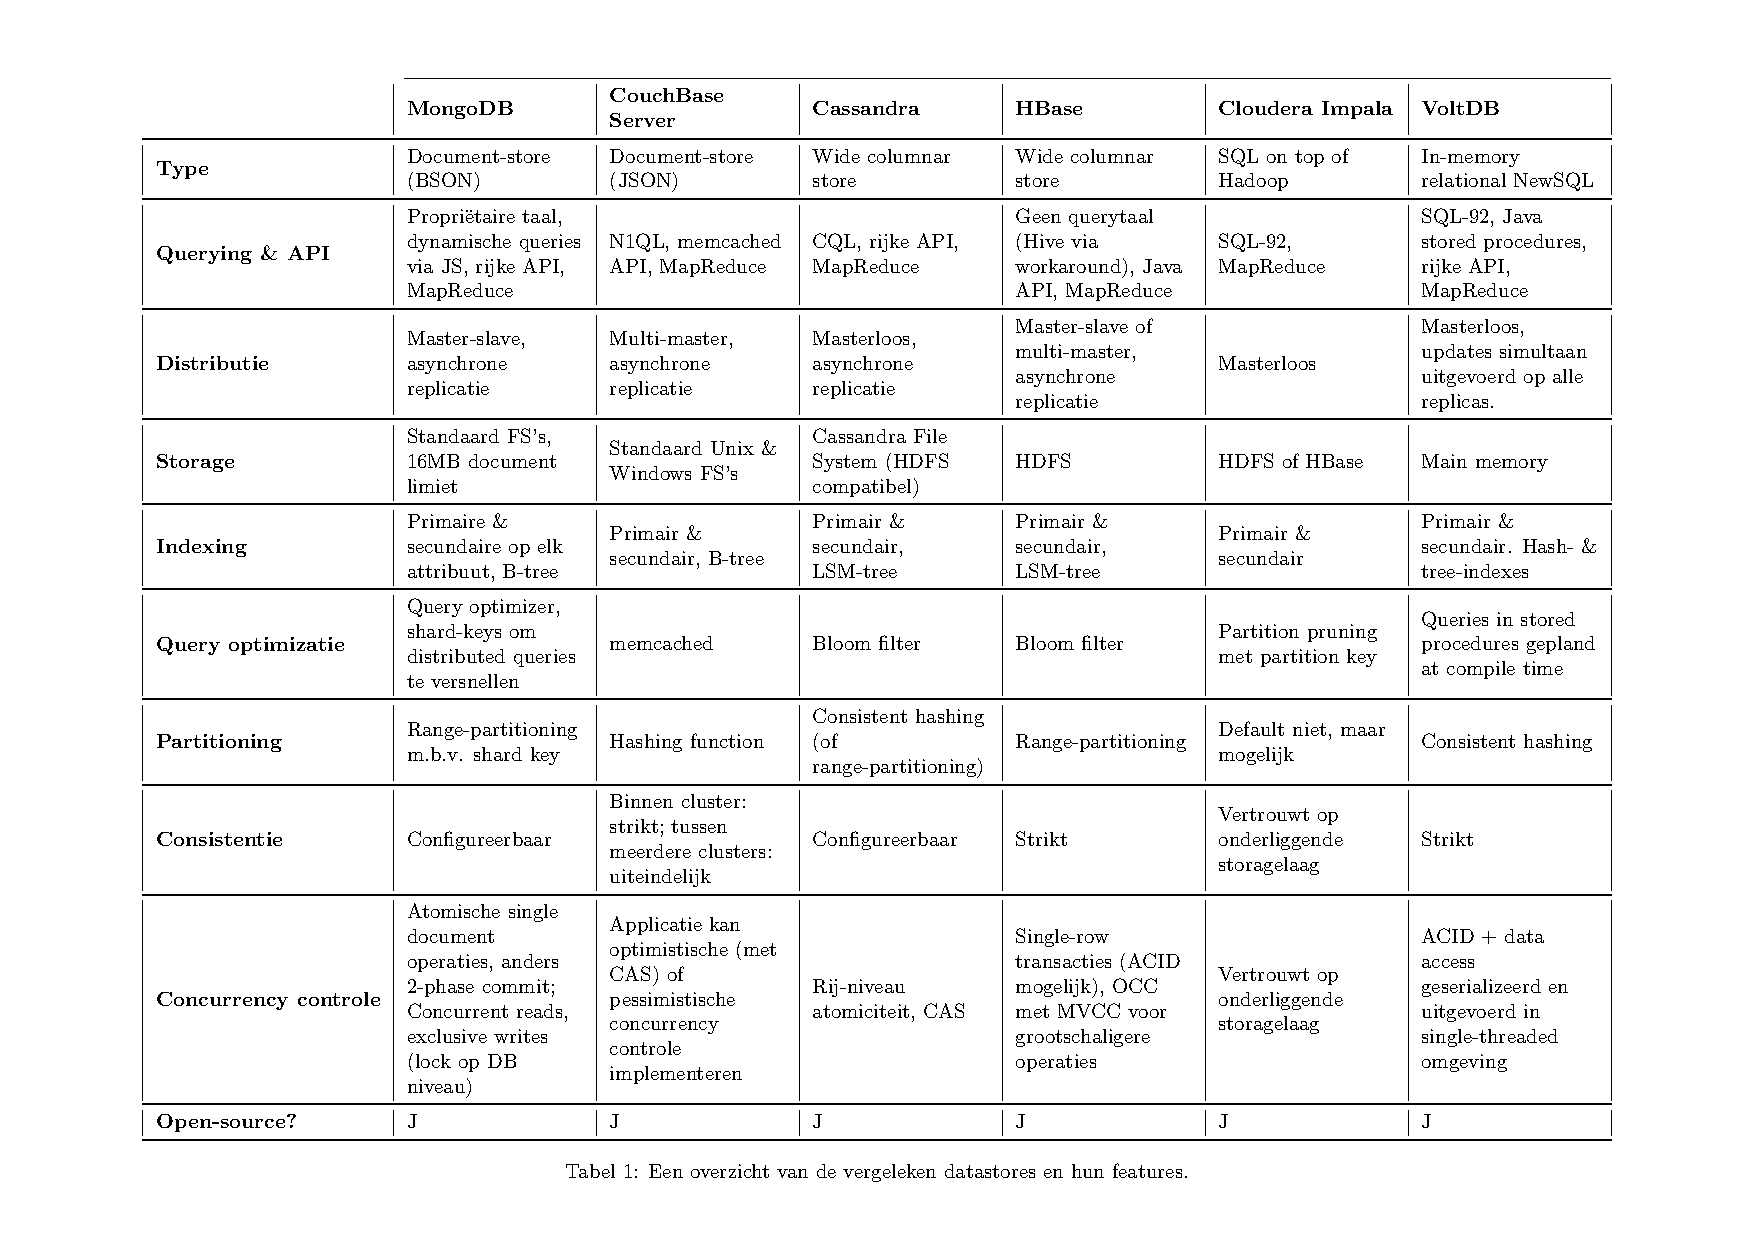
\includepdf[angle=90]{NoSQL_table_nl.pdf}
\label{survey_tabel}
\end{landscape}

\subsection{Document stores}

\paragraph{MongoDB}

MongoDB slaat gegevens op in BSON (binary JSON) documenten. Het systeem biedt krachtige ondersteuning voor indices, vooral door de mogelijkheid om secundaire indices van een brede waaier van types te defini\"eren op alle attributen, zoals in het relationele model. Deze indices zijn gebouwd op B-trees \cite{mongodb_indexes}. Om denormalizatie te bevorderen, kunnen documenten geneste documenten en arrays bevatten. Zo zijn joins ook overbodig in de query taal.\\
De bestandsgrootte is beperkt tot 16 MB, om te voorkomen dat \'e\'en enkel document buitensporig veel RAM of bandbreedte opeist. Om grotere bestanden te bewaren, kan het ingebouwde GridFS (dat integenstelling tot wat de naam doet vermoeden, geen volwaardig file system is) automatisch bestanden opsplitsen in kleinere delen en deze delen als aparte documenten bewaren, zonder dat de gebruiker zich hierom moet bekommeren.\\
MongoDB biedt API's in zeer vele programmeertalen en de functionaliteit om het equivalent van SQL \texttt{WHERE}-clausules te defini\"eren als javascript uitdrukkingen. MongoDB vertaalt deze vervolgens naar een eigen, interne en afgeschermde query taal \cite{grolinger2013data}. De query optimizer van MongoDB verwerkt queries en kiest voor elke query een zo effici\"ent mogelijk uitvoeringsplan gegeven de beschikbare indices. Deze plannen worden gecached als er meerdere goede alternatieven zijn en kunnen geherevalueerd worden naarmate de gegevensset in de databank evolueert.\\
Qua consistentie laat MongoDB de keuze tussen uiteindelijke en strikte consistentie. Strikte consistentie is mogelijk door ofwel enkel te lezen van de master node (die de meest up-to-date versie van de data heeft) of na schrijfopdrachten te wachten tot alle replica's bevestigd hebben alvorens verder te gaan. De eerste optie introduceert een bottleneck bij het lezen van data, de tweede verhoogt de latentie van schrijfopdrachten.\\
MongoDB repliceert data asynchroon en partitioneert in ranges: nodes zijn verantwoordelijk voor ranges van keys. Dit zorgt voor snelle range queries, maar kan hotspots en load-balancingproblemen veroorzaken. Dankzij een master-slave struktuur kan MongoDB updates gemakkelijk naar de juiste replica's doorverwijzen.
Op het gebied van concurrency controle biedt MongoDB atomiciteit binnen documenten en reader-writer locks. 
%TODO beter woord dan locken
Bij schrijfopdrachten de databank locken heeft een zware impact op de performantie in scenario's waar veel geschreven moet worden.\\\\
Kortom, MongoDB bewaart BSON-bestanden op een zeer toegankelijke manier met flexibele query- en indexeringsmechanismes. De concurrency- en consistentiemodellen daarentegen vertonen enkele nadelen.

\paragraph{Couchbase Server}

Couchbase, het resultaat van de fusie tussen CouchDB en Membase, slaat gegevens op in JSON documenten. Het hanteert het memcached protocol om een gedistribueerde cache en is bedoeld voor zeer interactieve toepassingen met hoge vereisten op gebied van latentie \cite{grolinger2013data}\cite{couchbase_about}.
De JSON documenten kunnen genest zijn en kunnen doorzocht worden met een uitgebreide, SQL-achtige taal, N1QL (op het moment van schrijven is dit wel nog steeds een developer preview, uitgebracht in januari 2015) \cite{couchbase_n1ql}.
Net als MongoDB kunnen primaire en secundaire indices gedefinieerd worden en zijn deze gestoeld op B-trees \cite{couchbase_index}.\\
Binnen \'e\'en cluster zijn transacties strikt consistent, maar tussen meerder clusters slechts uiteindelijk consistent.\\
CouchBase biedt gebruikers de keuze tussen optimistische (m.b.v. compare-and-swap) en pessimistische (m.b.v. 'finegrained locking') concurreny controle.\\\\
Dankzij zijn flexibele datamodel, caching en concurrency controle, past CouchBase goed voor toepassingen die snelle en intensieve interactieve vergen tussen gebruiker en data.

\subsection{Columnar stores}

\paragraph{Cassandra}

Cassandra werd oorspronkelijk ontwikkeld voor intern gebruik bij Facebook maar is later als Apache opensourceproject publiekelijk beschikbaar gemaakt. Het combineert het datamodel van Google's BigTable systeem met de architectuur en distributiestrategie van Amazons DynamoDB. Het is gericht op flexibele, quasipermanent beschikbare opslag van zeer grote datasets op goedkope standaardhardware, met daarenboven hoge througput voor schrijfopdrachten zonder effici\"entie bij leesopdrachten op te offeren \cite{borthakur2011apache}.\\
Sinds zijn ontstaan is Cassandra wel op enkele vlakken afgeweken van het BigTable-model \cite{cassandra_then&now}, in die zin dat het nu tabellen en samengestelde kolommen
%TODO betere vertaling voor composite columns?
biedt, evenals een eigen query taal, CQL \cite{cassandra_CQL}. CQL vertoont op het gebied van syntax en functionaliteit sterke gelijkenissen met SQL, maar is toch sterk beperkt. Zo biedt het bijvoorbeeld geen \texttt{JOIN}-clausule, en zijn \texttt{WHERE}-clausules aan sterke voorwaarden onderhevig. Cassandra moedigt het samenbewaren van gegevens die samen opgevraagd worden sterk aan en ondersteunt denormalizatie met features zoals collection types.\\
Cassandra heeft indexeringsmechanismes and implementeert deze met log-structured merge trees, met hogere schrijfthroughput als gevolg.
Net als BigTable biedt Cassandra ook Bloom filters: een effici\"ent probabilistische mechanisme om te voorspellen of een object in een verzameling zit (in dit geval, of een key in een tabel ligt, dat het aantal nodeloze table scans beduidend kan inperken \cite{mullin1983second}.\\
Om lineair in het aantal ingeschakelde nodes te kunnen schalen naar zeer grote datasets, opereert Cassandra op een volledig hi\"erarchieloze wijze. Vanuit het perspectief van het CAP-theorema, spitst Cassandra zich toe op availability en partition tolerance, ten koste van onmiddellijke consistentie. Het consistentieniveau kan wel per query door de gebruiker bepaald worden, zoals later verduidelijkt wordt. Hoge beschikbaarheid en tolerantie voor fouten bereikt Cassandra door asynchroon data te repliceren over verschillende nodes, met consistent hashing en virtuele nodes om frequent komen-en-gaan en incrementeel toevoegen van nodes op te vangen. Het aantal replica's kan de gebruiker zelf kiezen. Bovendien voorziet Cassandra ook interdatacenterreplicatie, om zelfs het falen van volledige datacenters op te vangen \cite{decandia2007dynamo} \cite{lakshman2010cassandra} \cite{cassandra_then&now}.\\
Bij lees- en schrijfopdrachten kan de gebruiker een quorum specifi\"eren. Hoewel Cassandra met uiteindelijke consistentie voor het oog ontworpen werd, is onmiddellijke consistentie mits een juiste keuze van de quorum dus ook een optie.\\
Op het gebied van concurrency controle garandeert Cassandra atomiciteit binnen rijen en serializeerbare \textit{lightweight transactions}, eigenlijk compare-and-set functionaliteit, voor grotere operaties.
\\\\
Samengevat biedt Cassandra redelijk flexibele datamodellering met (licht beperkte) query- en indexeringsmechanismen via de CQL-interface. Het sterkste punt is echter dat Cassandra incrementeel schaalt naar enorme datasets, dankzij uitvoerige replicatie- en foutverwerkingsfeatures.

\paragraph{HBase}

Apache HBase is een opensource datastore gebaseerd op het datamodel van Google BigTable, die draait bovenop het Hadoop Distributed File System (HDFS) in plaats van het Google File System (GFS).\\
Sinds z'n lancering heeft HBase verschillende secundaire indexeringsmechanismes verworven. Deze zijn ook gebaseerd op LSM trees en daarnaast biedt ook HBase Bloom filters \cite{borthakur2011apache}\cite{hbase_schema}. HBase heeft een Java API, maar zonder SQL-achtige geavanceerde querytaal. Hierbij moet wel opgemerkt worden dat een omweg via Apache Hive, een ander data-opslag en -analyseproject \cite{apache_hive}, en de bijhorende querytaal HiveQL dit probleem kan verhelpen. Dankzij de HDFS-fundering can HBase vlot fungeren als in- en output voor MapReduce taken.\\
HBase partitioneert data net als BigTable in ranges en repliceert gegevens op ofwel master-slave of multi-master wijze. Leesopdrachten worden echter niet gedistribueerd: er is slechts 1 server die instaat voor elke rij. De replica's zijn enkel bestemd voor het herstellen van fouten.\\
De sterke punten van HBase zijn de sterke consistentie, een rariteit in de NoSQL-wereld, en concurrency-model: ACID transactions binnen rijen en optimistische, multi-version concurrency controle voor grootschaligere operaties \cite{hbase_acid}\cite{grolinger2013data}\cite{borthakur2011apache}.\\

Kort samengevat laat HBase gebruikers toe flexibel data te modelleren en is het systeem vooral nuttig wanneer het startpunt een dataset in HDFS is en MapReduce-compatibiliteit een prioriteit is. HBase schaalt goed naar zeer grote datasets en beschikt over uitstekende concurrency- en consistentie-eigenschappen.

\subsection{NewSQL} 

\paragraph{VoltDB}

VoltDB is een relationele, gedistribueerde in-memory databank, die als doel heeft de garanties van klassieke SQL-stores te koppelen met de schaalbaarheid van NoSQL-systemen, en bovendien aan zeer hoge snelheden te functioneren \cite{stonebraker2013voltdb}.\\
VoltDB bewaart gegevens in het traditionele relationele model, maar gerepliceerd en gepartitioneerd (met consistent hashing) over verschillende nodes \cite{grolinger2013data}. De data is doorzoekbaar via een (groeiende) subset van SQL-92 \cite{voltdb2010voltdb}. Queries worden bij voorkeur gedefinieerd als stored procedures in Java, met daarin ingebed de SQL uitdrukkingen. VoltDB ondersteunt primaire en secundaire indices en laat de gebruiker de keuze tussen hash- en boomindices \cite{voltdb_indexes}. VoltDB plant en optimaliseert de queries in stored procedures offline tijdens het compileren \cite{voltdb_query_plans}.\\
Omdat VoltDB volledig op RAM geheugen vertrouwt, is het duur om te schalen naar datavolumes in de grootorde van meerdere petabytes, maar VoltDB kan data exporteren naar andere, meer geschikte databanksystemen zoals columnaire NoSQL systemen.\\
Vooral op het gebied van concurrency controle onderscheidt VoltDB zich van andere systemen: transacties voldoen aan de ACID-eigenschappen en worden simultaan op alle replica's uitgevoerd. Het geheugen is in blokken verdeeld, die elk statisch toegewezen zijn aan \'e\'en enkele, single-threaded core. Een globale controller serializeert alle transacties waarbij meerdere nodes betrokken zijn tot een sequentie van enkelvoudige transacties en voegt deze in de transaction queues van de betrokken nodes. Op deze manier maakt VoltDB locking en latching technieken overbodig. De durability uit ACID bereikt VoltDB door op regelmatige basis snapshots van de databank in het geheugen te nemen en deze op schijf op te slaan.\\

Kort samengevat is VoltDB een relationele databank in main memory die schaalt tot relatief grote datasets, met zeer snelle SQL-query-capaciteiten en ACID-transacties. Het is bijgevolg meer geschikt voor rekenintensieve toepassingen die niet overdreven veel data verwerken, maar wel zeer lage latentie vereisen.

\paragraph{Cloudera Impala}

Cloudera Impala is een gedistribueerde SQL-machine die draait bovenop de Hadoopstack, ofwel op HDFS of op HBase \cite{cloudera_impala}. Ze is specfiek bedoeld voor analytisch gebruik, met een focus op het leveren van real-time query-capaciteiten eerder dan op hoge throughput bij schrijfopdrachten.\\
Opgeslagen data is toegankelijk via een subset van SQL-92.\\
Impala's architectuur is bijna perfect symmetrisch gedistribueerd: alle nodes voeren hetzelfde \texttt{impalad}-proces uit, dat de belangrijkste databankfunctionaliteiten verzorgt. Elke node kan als startpunt fungeren voor een query en zal vervolgens de query in kwestie co\"ordineren. Twee processen lopen daarentegen op \'e\'en enkele (niet noodzakelijk dezelfde) node in het cluster; zij staan in voor boekhoudkundige taken en doorgeven van wijzingen aan metadata doorheen het cluster \cite{impala_components}.\\
In tegenstelling tot voorgaande opties partitioneert Impala rijen niet automatisch. De gebruiker krijgt wel de keuze hiertoe, voor in het geval de hoeveelheid gegevens hierom zou vragen \cite{impala_partitioning}.\\
Impala beschikt over een zeer effici\"ente I/O-laag die schijf- en CPU-gebruik te allen tijde hoog houdt, wat resulteert in aanzienlijk snellere prestaties dan andere SQL-on-Hadoop oplossingen zoals Apache Hive \cite{floratou2014sql}. Het inherente nadeel is echter dat de volledige dataset moet passen in het totale werkgeheugen van het cluster waarin Impala draait. Dit beperkt enigszins de grootte van datasets diet Impala kan verwerken, ondanks de schaalbaarheid van de onderliggende Hadooplaag.\\
Omwille van z'n analytische doeleinden heeft Impala geen uitvoerige mechanismes voor concurrency controle, maar vertrouwt hiervoor op het onderliggende opslagsysteem. Gezien de uitstekende concurrency-eigenschappen van HBase vormt dit niet noodzakelijk een probleem.